\documentclass[border=10pt]{standalone}

\usepackage{tikz}
\usepackage{amsmath}

\usetikzlibrary{
    positioning,
    arrows.meta,
    fit,
    backgrounds,
    shapes.geometric,
    calc
}

\pagestyle{empty}
% ============================================================================
% PART II: UPDATED FEATURES -> FUSION -> LOSSES
% ============================================================================
\begin{document}
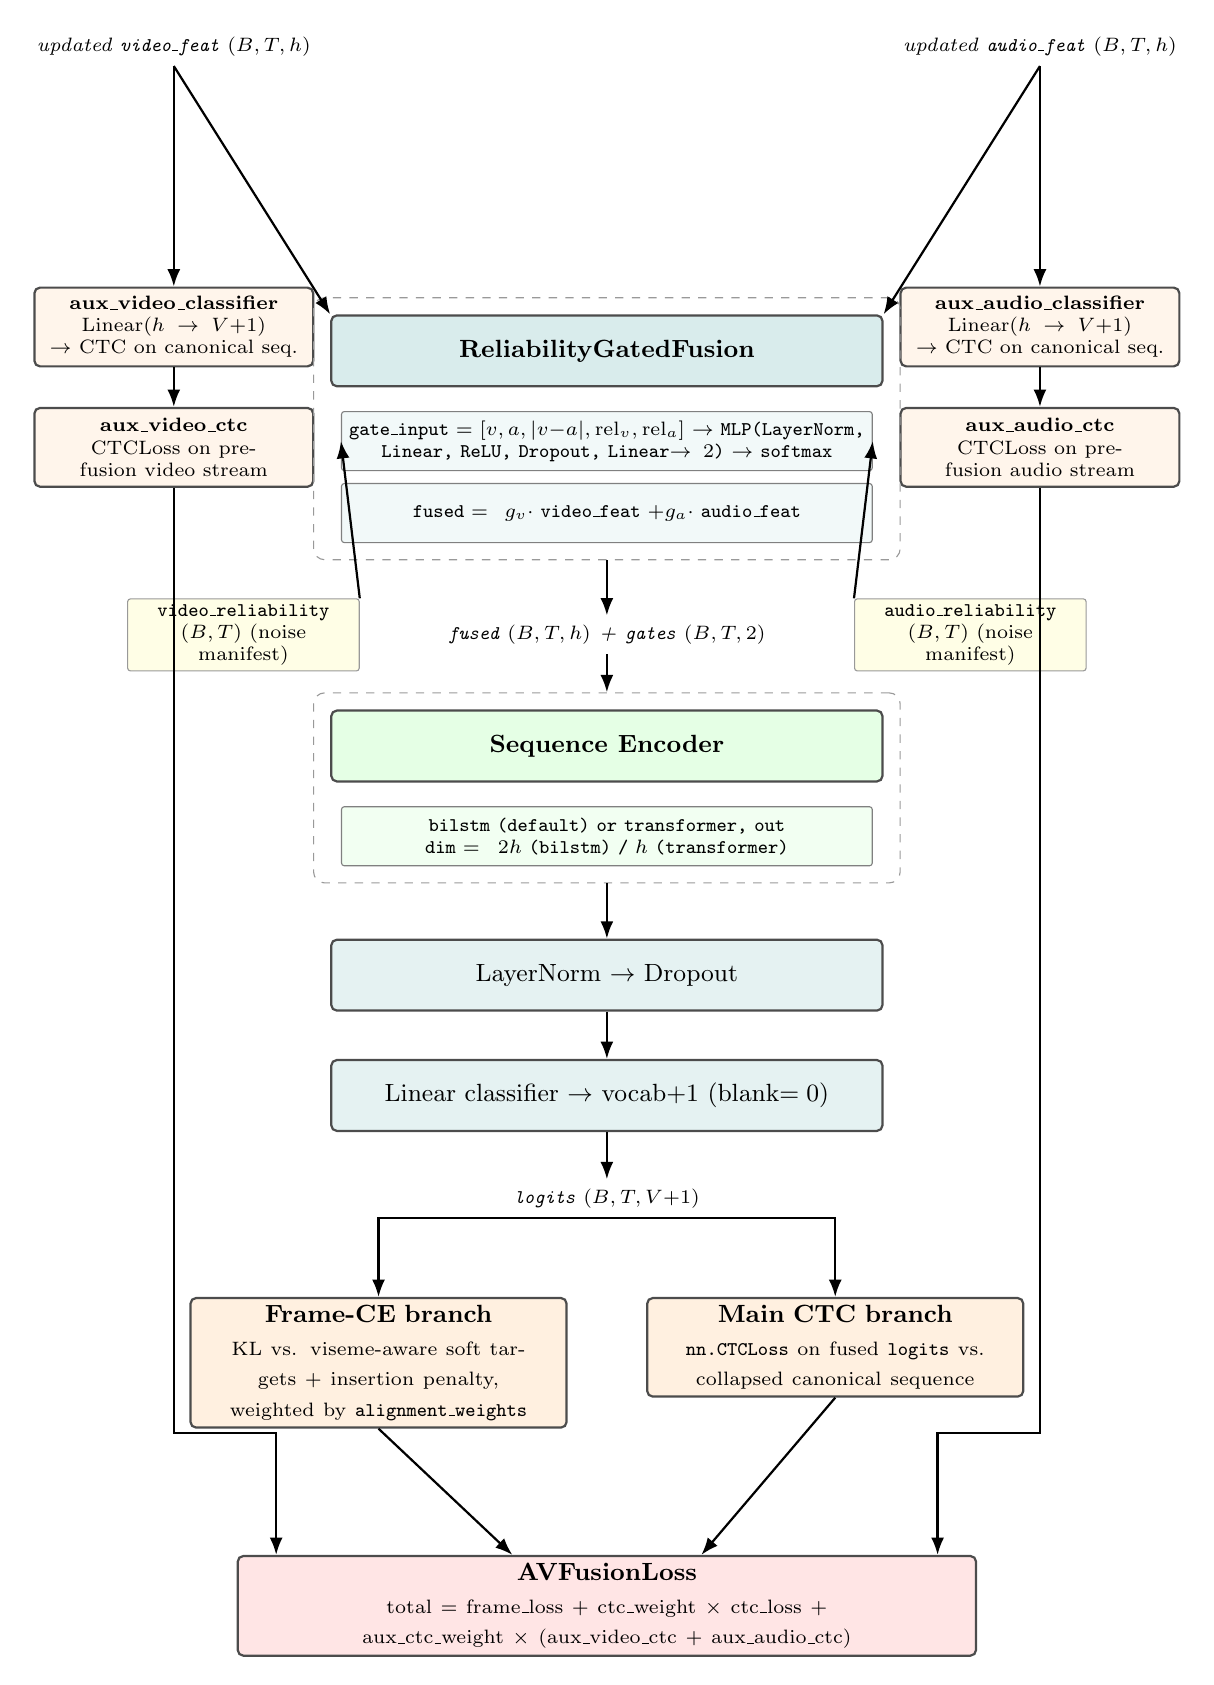
\begin{tikzpicture}[
    font=\small,
    node distance=5mm and 10mm,
    centerblock/.style={
        rectangle, draw=black!70, thick, rounded corners=2pt,
        fill=teal!10, minimum width=70mm, minimum height=9mm,
        align=center, inner sep=2.5pt
    },
    subblock/.style={
        rectangle, draw=black!50, rounded corners=1pt,
        fill=teal!5, minimum width=66mm, minimum height=7.5mm,
        align=center, font=\scriptsize\ttfamily, inner sep=2pt,
        text width=66mm
    },
    smallbranch/.style={
        rectangle, draw=black!70, thick, rounded corners=2pt,
        fill=orange!8, minimum width=34mm, minimum height=10mm,
        align=center, inner sep=2pt, font=\scriptsize,
        text width=34mm
    },
    branch/.style={
        rectangle, draw=black!70, thick, rounded corners=2pt,
        fill=orange!12, minimum width=46mm, minimum height=11mm,
        align=center, inner sep=2.5pt, text width=46mm
    },
    iolabel/.style={
        rectangle, draw=none, fill=none, align=center, font=\scriptsize\itshape
    },
    sidelabel/.style={
        rectangle, draw=black!40, fill=yellow!10, rounded corners=1pt,
        align=center, font=\scriptsize, inner sep=2pt
    },
    groupbox/.style={
        rectangle, draw=black!40, dashed, rounded corners=4pt, inner sep=6pt
    },
    arr/.style={-{Latex[length=2.2mm]}, thick},
    every label/.style={font=\scriptsize}
]

% Split-point inputs
\node[iolabel] (v_feat2) at (-55mm,0) {updated \texttt{video\_feat} $(B,T,h)$};
\node[iolabel] (a_feat2) at (55mm,0)
    {updated \texttt{audio\_feat} $(B,T,h)$};

% Auxiliary branches are deliberately placed far outside the central fusion path.
\node[smallbranch, below=28mm of v_feat2] (aux_v)
    {\textbf{aux\_video\_classifier}\\Linear$(h\to V{+}1)$\\$\to$ CTC on canonical seq.};
\node[smallbranch, below=28mm of a_feat2] (aux_a)
    {\textbf{aux\_audio\_classifier}\\Linear$(h\to V{+}1)$\\$\to$ CTC on canonical seq.};
\node[smallbranch, below=5mm of aux_v] (aux_v_ctc)
    {\textbf{aux\_video\_ctc}\\CTCLoss on pre-fusion video stream};
\node[smallbranch, below=5mm of aux_a] (aux_a_ctc)
    {\textbf{aux\_audio\_ctc}\\CTCLoss on pre-fusion audio stream};

% Central fusion block, well below the split point
\node[centerblock, below=34mm of $(v_feat2)!0.5!(a_feat2)$, fill=teal!15]
    (fusion_title) {\textbf{ReliabilityGatedFusion}};
\node[subblock, below=3mm of fusion_title] (fusion_gate)
    {gate\_input $=[v,a,|v{-}a|,\mathrm{rel}_v,\mathrm{rel}_a]$ $\to$ MLP(LayerNorm, Linear, ReLU, Dropout, Linear$\to2$) $\to$ softmax};
\node[subblock, below=1.5mm of fusion_gate] (fusion_combine)
    {\texttt{fused} $=g_v\cdot$ video\_feat $+g_a\cdot$ audio\_feat};
\node[groupbox, fit=(fusion_title)(fusion_gate)(fusion_combine)] (fusionbox) {};

% Main encoder pipeline
\node[iolabel, below=7mm of fusionbox] (fused_lbl)
    {\texttt{fused} $(B,T,h)$ + \texttt{gates} $(B,T,2)$};
% Reliability metadata sits beside the compact fused/gates label,
% between the fusion block and the sequence encoder.
\node[sidelabel, text width=28mm, anchor=east] (vrel) at ([xshift=-10mm]fused_lbl.west)
    {\texttt{video\_reliability}\\$(B,T)$ (noise manifest)};
\node[sidelabel, text width=28mm, anchor=west] (arel) at ([xshift=10mm]fused_lbl.east)
    {\texttt{audio\_reliability}\\$(B,T)$ (noise manifest)};
\node[centerblock, below=7mm of fused_lbl, fill=green!10] (enc_title)
    {\textbf{Sequence Encoder}};
\node[subblock, below=3mm of enc_title, fill=green!5] (bilstm)
    {\texttt{bilstm} (default) or \texttt{transformer}, out dim $=2h$ (bilstm) / $h$ (transformer)};
\node[groupbox, fit=(enc_title)(bilstm)] (encbox) {};
\node[centerblock, below=7mm of encbox] (norm) {LayerNorm $\to$ Dropout};
\node[centerblock, below=6mm of norm] (classifier) {Linear classifier $\to$ vocab$+1$ (blank$=0$)};
\node[iolabel, below=6mm of classifier] (logits_lbl) {\texttt{logits} $(B,T,V{+}1)$};

% Main loss branches, widely separated
\node[branch, below=10mm of logits_lbl, xshift=-29mm] (framece)
    {\textbf{Frame-CE branch}\\[1pt] \scriptsize KL vs. viseme-aware soft targets + insertion penalty, weighted by \texttt{alignment\_weights}};
\node[branch, below=10mm of logits_lbl, xshift=29mm] (ctc)
    {\textbf{Main CTC branch}\\[1pt] \scriptsize \texttt{nn.CTCLoss} on fused \texttt{logits} vs. collapsed canonical sequence};

% Total loss below the four branches; all arrows enter vertically from above.
\node[centerblock, below=18mm of $(framece.south)!0.5!(ctc.south)$,
      fill=red!10, minimum width=92mm, text width=92mm] (total)
    {\textbf{AVFusionLoss}\\[1pt] \scriptsize total $=$ frame\_loss $+$ ctc\_weight $\times$ ctc\_loss
     $+$ aux\_ctc\_weight $\times$ (aux\_video\_ctc $+$ aux\_audio\_ctc)};

% ------------------------------- Arrows --------------------------------------
% Feature -> auxiliary heads: route outward so the central fusion path stays clear.
\draw[arr] (v_feat2.south) -- (aux_v.north);
\draw[arr] (a_feat2.south) -- (aux_a.north);
\draw[arr] (aux_v.south) -- (aux_v_ctc.north);
\draw[arr] (aux_a.south) -- (aux_a_ctc.north);

% Feature -> fusion: clean inward diagonals, completely independent of the aux branches.
\draw[arr] (v_feat2.south) -- (fusion_title.north west);
\draw[arr] (a_feat2.south) -- (fusion_title.north east);

% Reliability inputs feed the fusion gate from their positions beside fused/gates.
\draw[arr] (vrel.north east) -- (fusion_gate.west);
\draw[arr] (arel.north west) -- (fusion_gate.east);
% Main forward path
\draw[arr] (fusionbox.south) -- (fused_lbl.north);
\draw[arr] (fused_lbl.south) -- (encbox.north);
\draw[arr] (encbox.south) -- (norm.north);
\draw[arr] (norm.south) -- (classifier.north);
\draw[arr] (classifier.south) -- (logits_lbl.north);

% Logits -> main loss branches
\draw[arr] (logits_lbl.south) -| (framece.north);
\draw[arr] (logits_lbl.south) -| (ctc.north);

% All four loss terms enter AVFusionLoss from above at separate x positions.
\draw[arr] (aux_v_ctc.south) -- ++(0,-120mm) -| ([xshift=-42mm,yshift=6mm]total.north) -- ([xshift=-42mm]total.north);
\draw[arr] (framece.south) -- ([xshift=-12mm]total.north);
\draw[arr] (ctc.south) -- ([xshift=12mm]total.north);
\draw[arr] (aux_a_ctc.south) -- ++(0,-120mm) -| ([xshift=42mm,yshift=6mm]total.north) -- ([xshift=42mm]total.north);

\end{tikzpicture}
\end{document}